
% ════════════════════════════════════════════
% 模型求解（5.1.4.模型求解.tex，三级子块）
% ════════════════════════════════════════════
\subsubsection{调度结果与费用结构}

基于上述模型，本节利用附件一数据在 Python 环境下调用线性规划求解器进行求解。核心参数为 $\Delta t=1/6$ h、$\eta=0.9$、$E_{\min}=1200$ kWh、$E_{\max}=10800$ kWh、$P_{\max}=5000$ kW，并按附录1给定 $E_0=6000$ kWh。求解得到微网在指定时间段的购电量及全天购电量和购电费如表\ref{tab:结果1-1}所示，储能设备在指定时段的充放电量及储电量如表\ref{tab:结果1-2}所示。

分时电价与最优购电功率的对应关系如图\ref{fig:结果1-2}所示。可以看到，购电功率主要集中在夜间低电价时段，用于在低价区间补充负荷缺口并为储能充电；在电价高峰时段购电功率明显下降，说明储能放电有效替代了高价购电。

负荷、光伏、净负荷与储能充放电功率的时序关系如图\ref{fig:结果1-3}所示。可以看出，光伏功率在白天形成明显高峰，使净负荷在午间大幅下降甚至转负，此时储能吸收光伏盈余进行充电；而在夜间与傍晚负荷高峰，储能放电填补净负荷缺口，购电功率相应减小。

\begin{figure}[H]
    \centering
    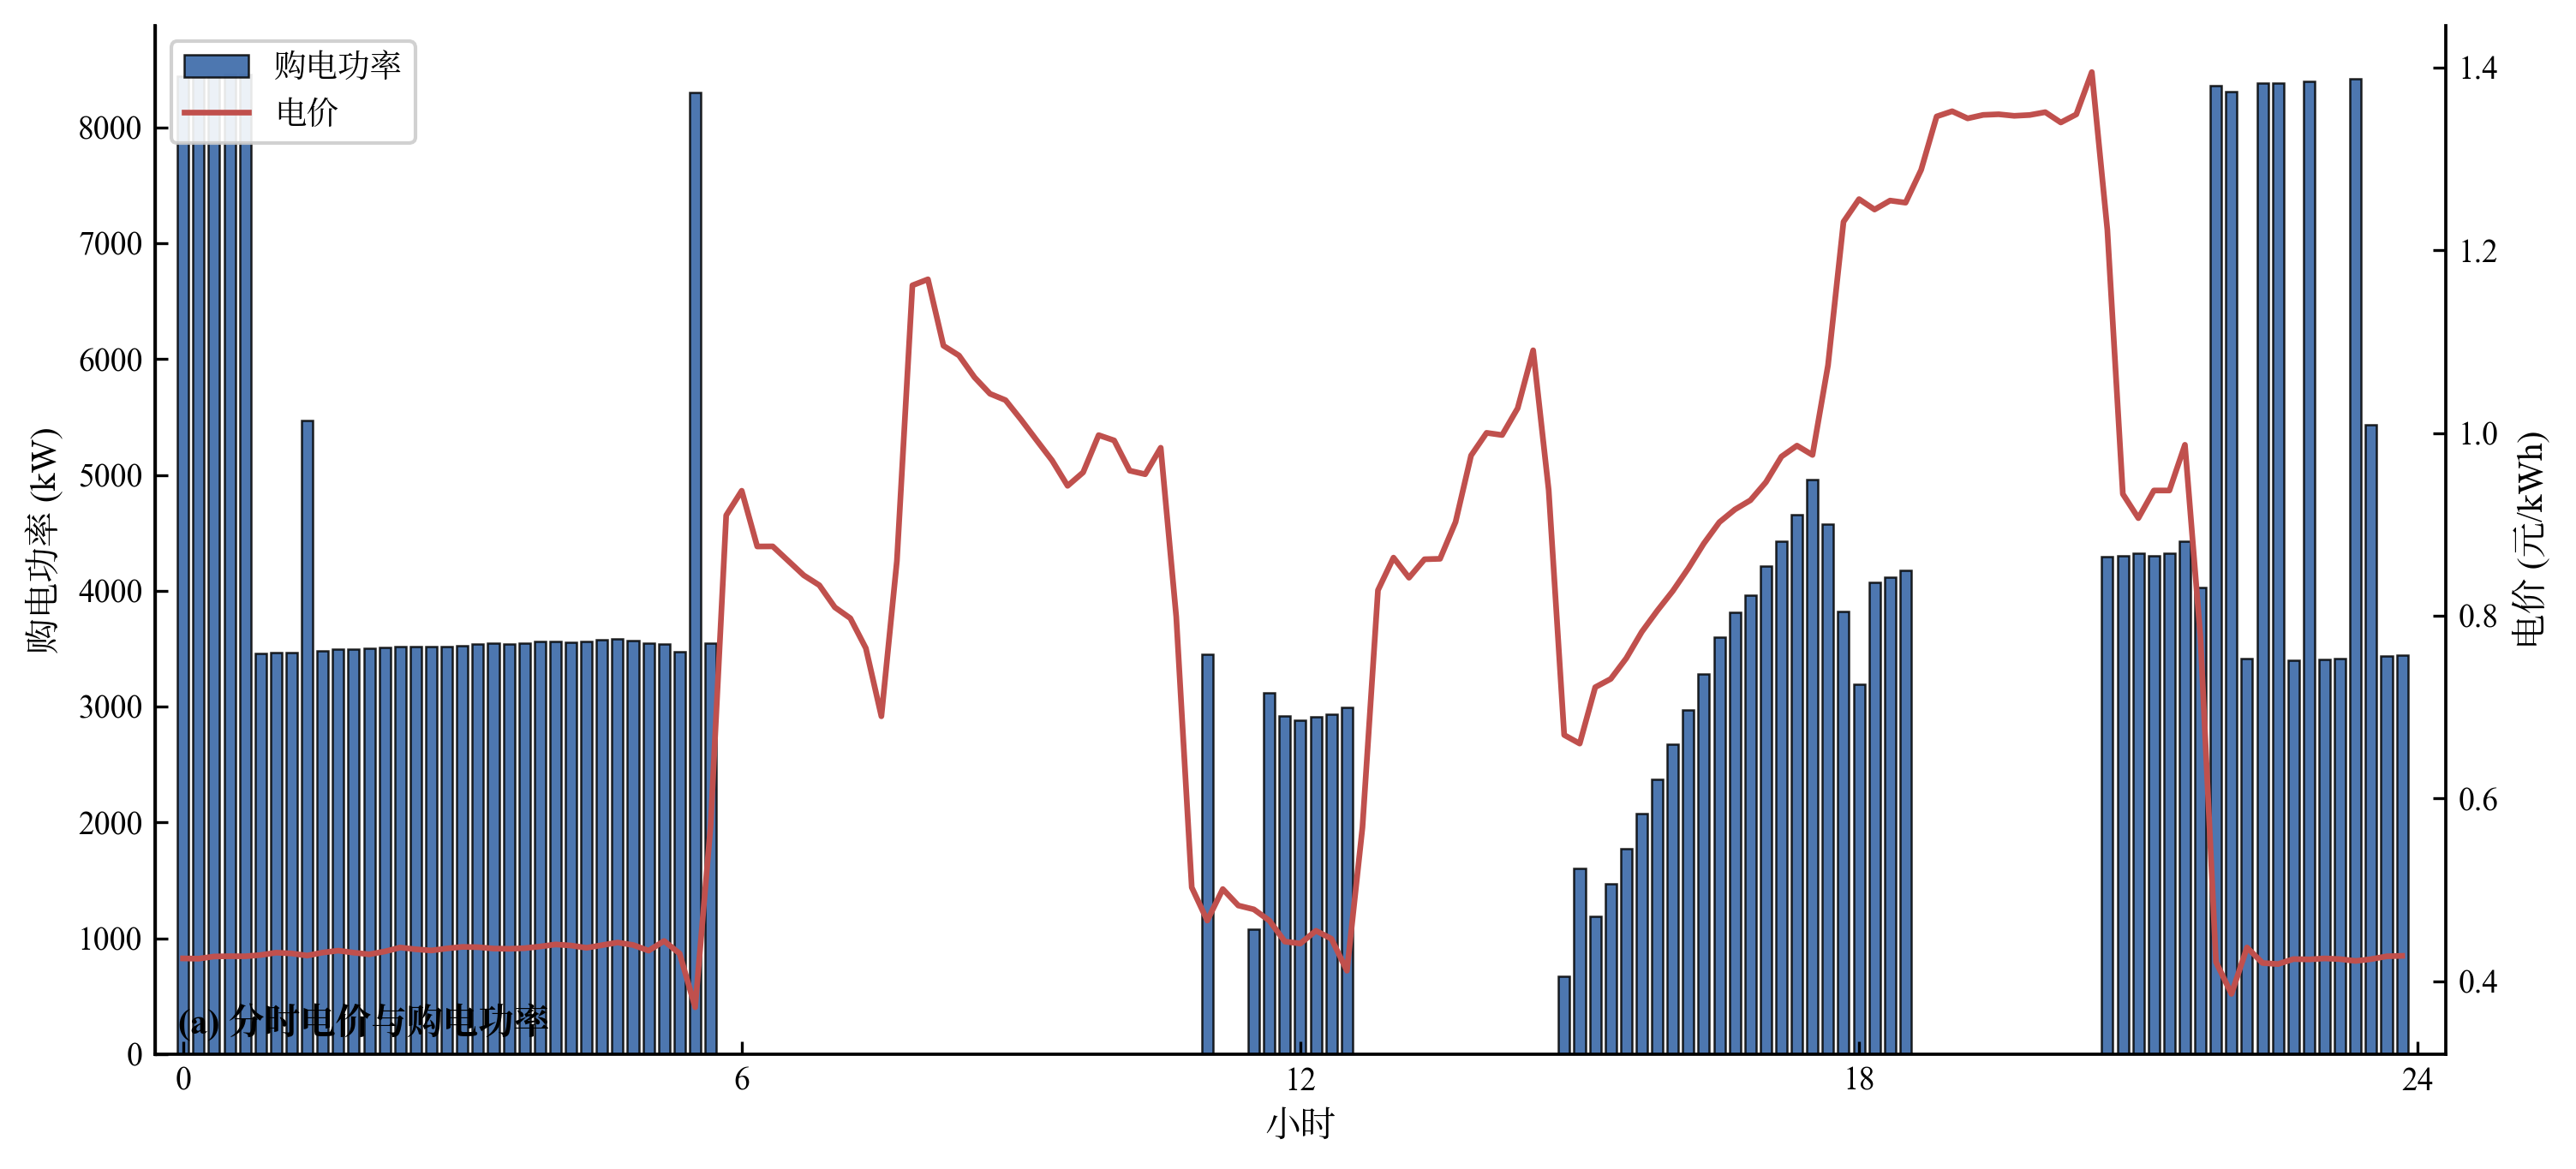
\includegraphics[width=0.65\textwidth]{求解/问题一/图片/图1-2_电价与购电策略.png}
    \caption{分时电价与最优购电功率}
    \label{fig:结果1-2}
\end{figure}

\begin{figure}[H]
    \centering
    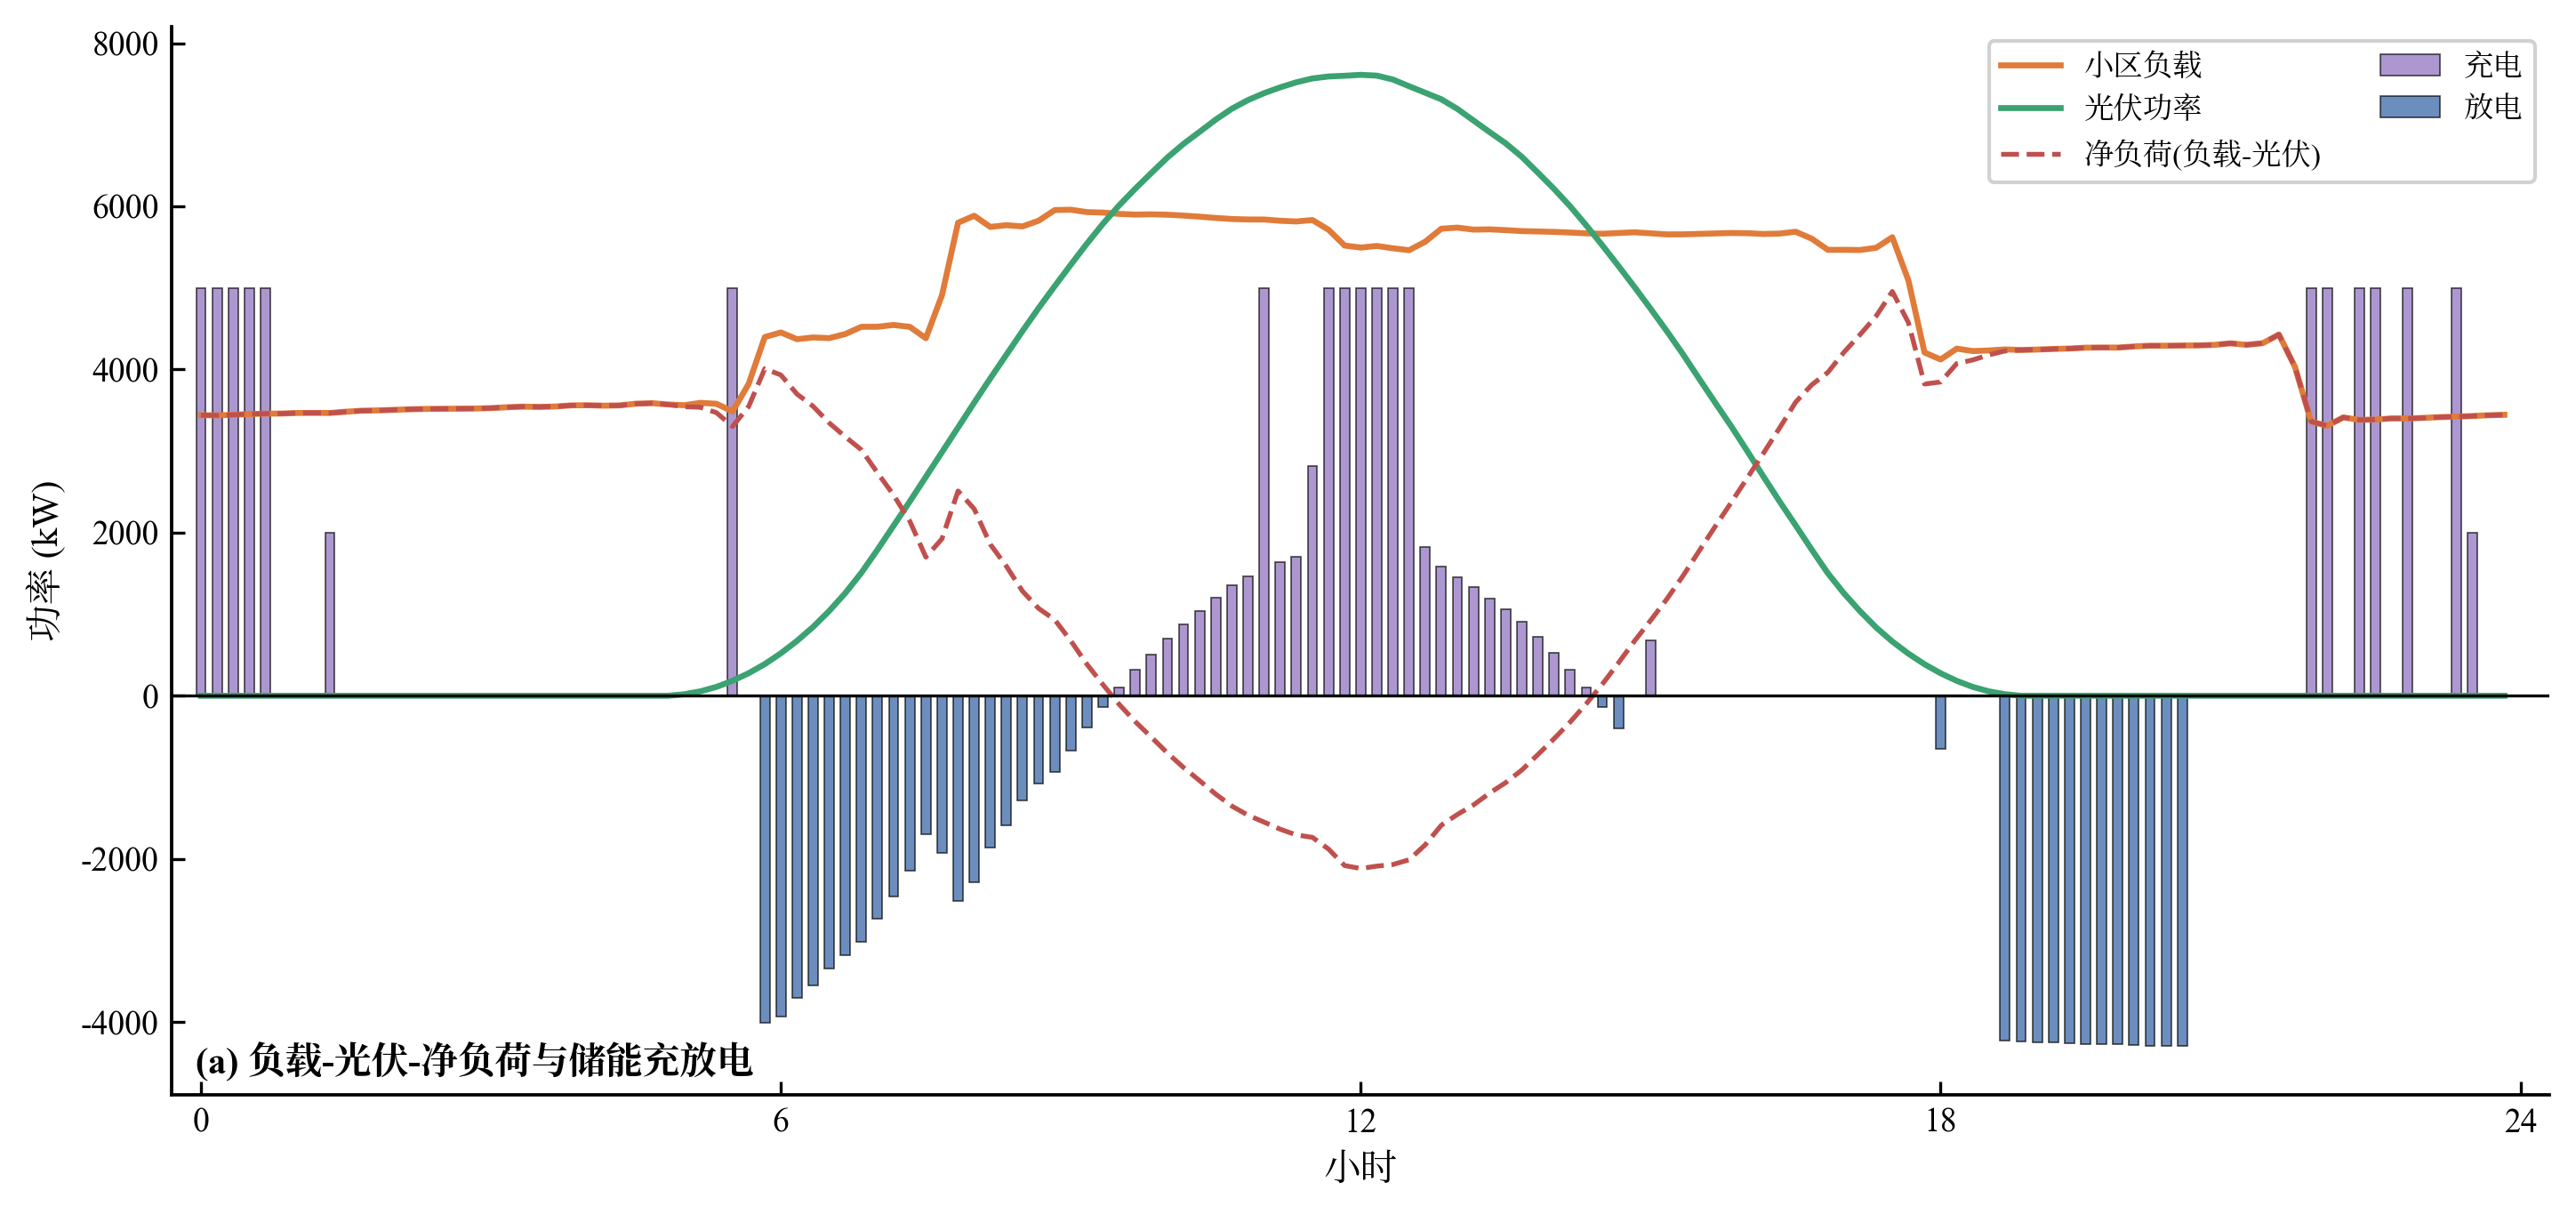
\includegraphics[width=0.65\textwidth]{求解/问题一/图片/图1-3_负荷光伏净负荷与充放电.png}
    \caption{负荷、光伏、净负荷与储能充放电功率}
    \label{fig:结果1-3}
\end{figure}

储能设备的荷电状态轨迹与充放电功率如图\ref{fig:结果1-4}所示。储能荷电状态全程维持在 $[1200,10800]$ kWh 约束区间内，且在 0:00 与 24:00 处均精确等于附录1给定的 6000 kWh；充放电功率始终不超过 5000 kW 的额定限值，验证了模型的可行性。

\begin{figure}[H]
    \centering
    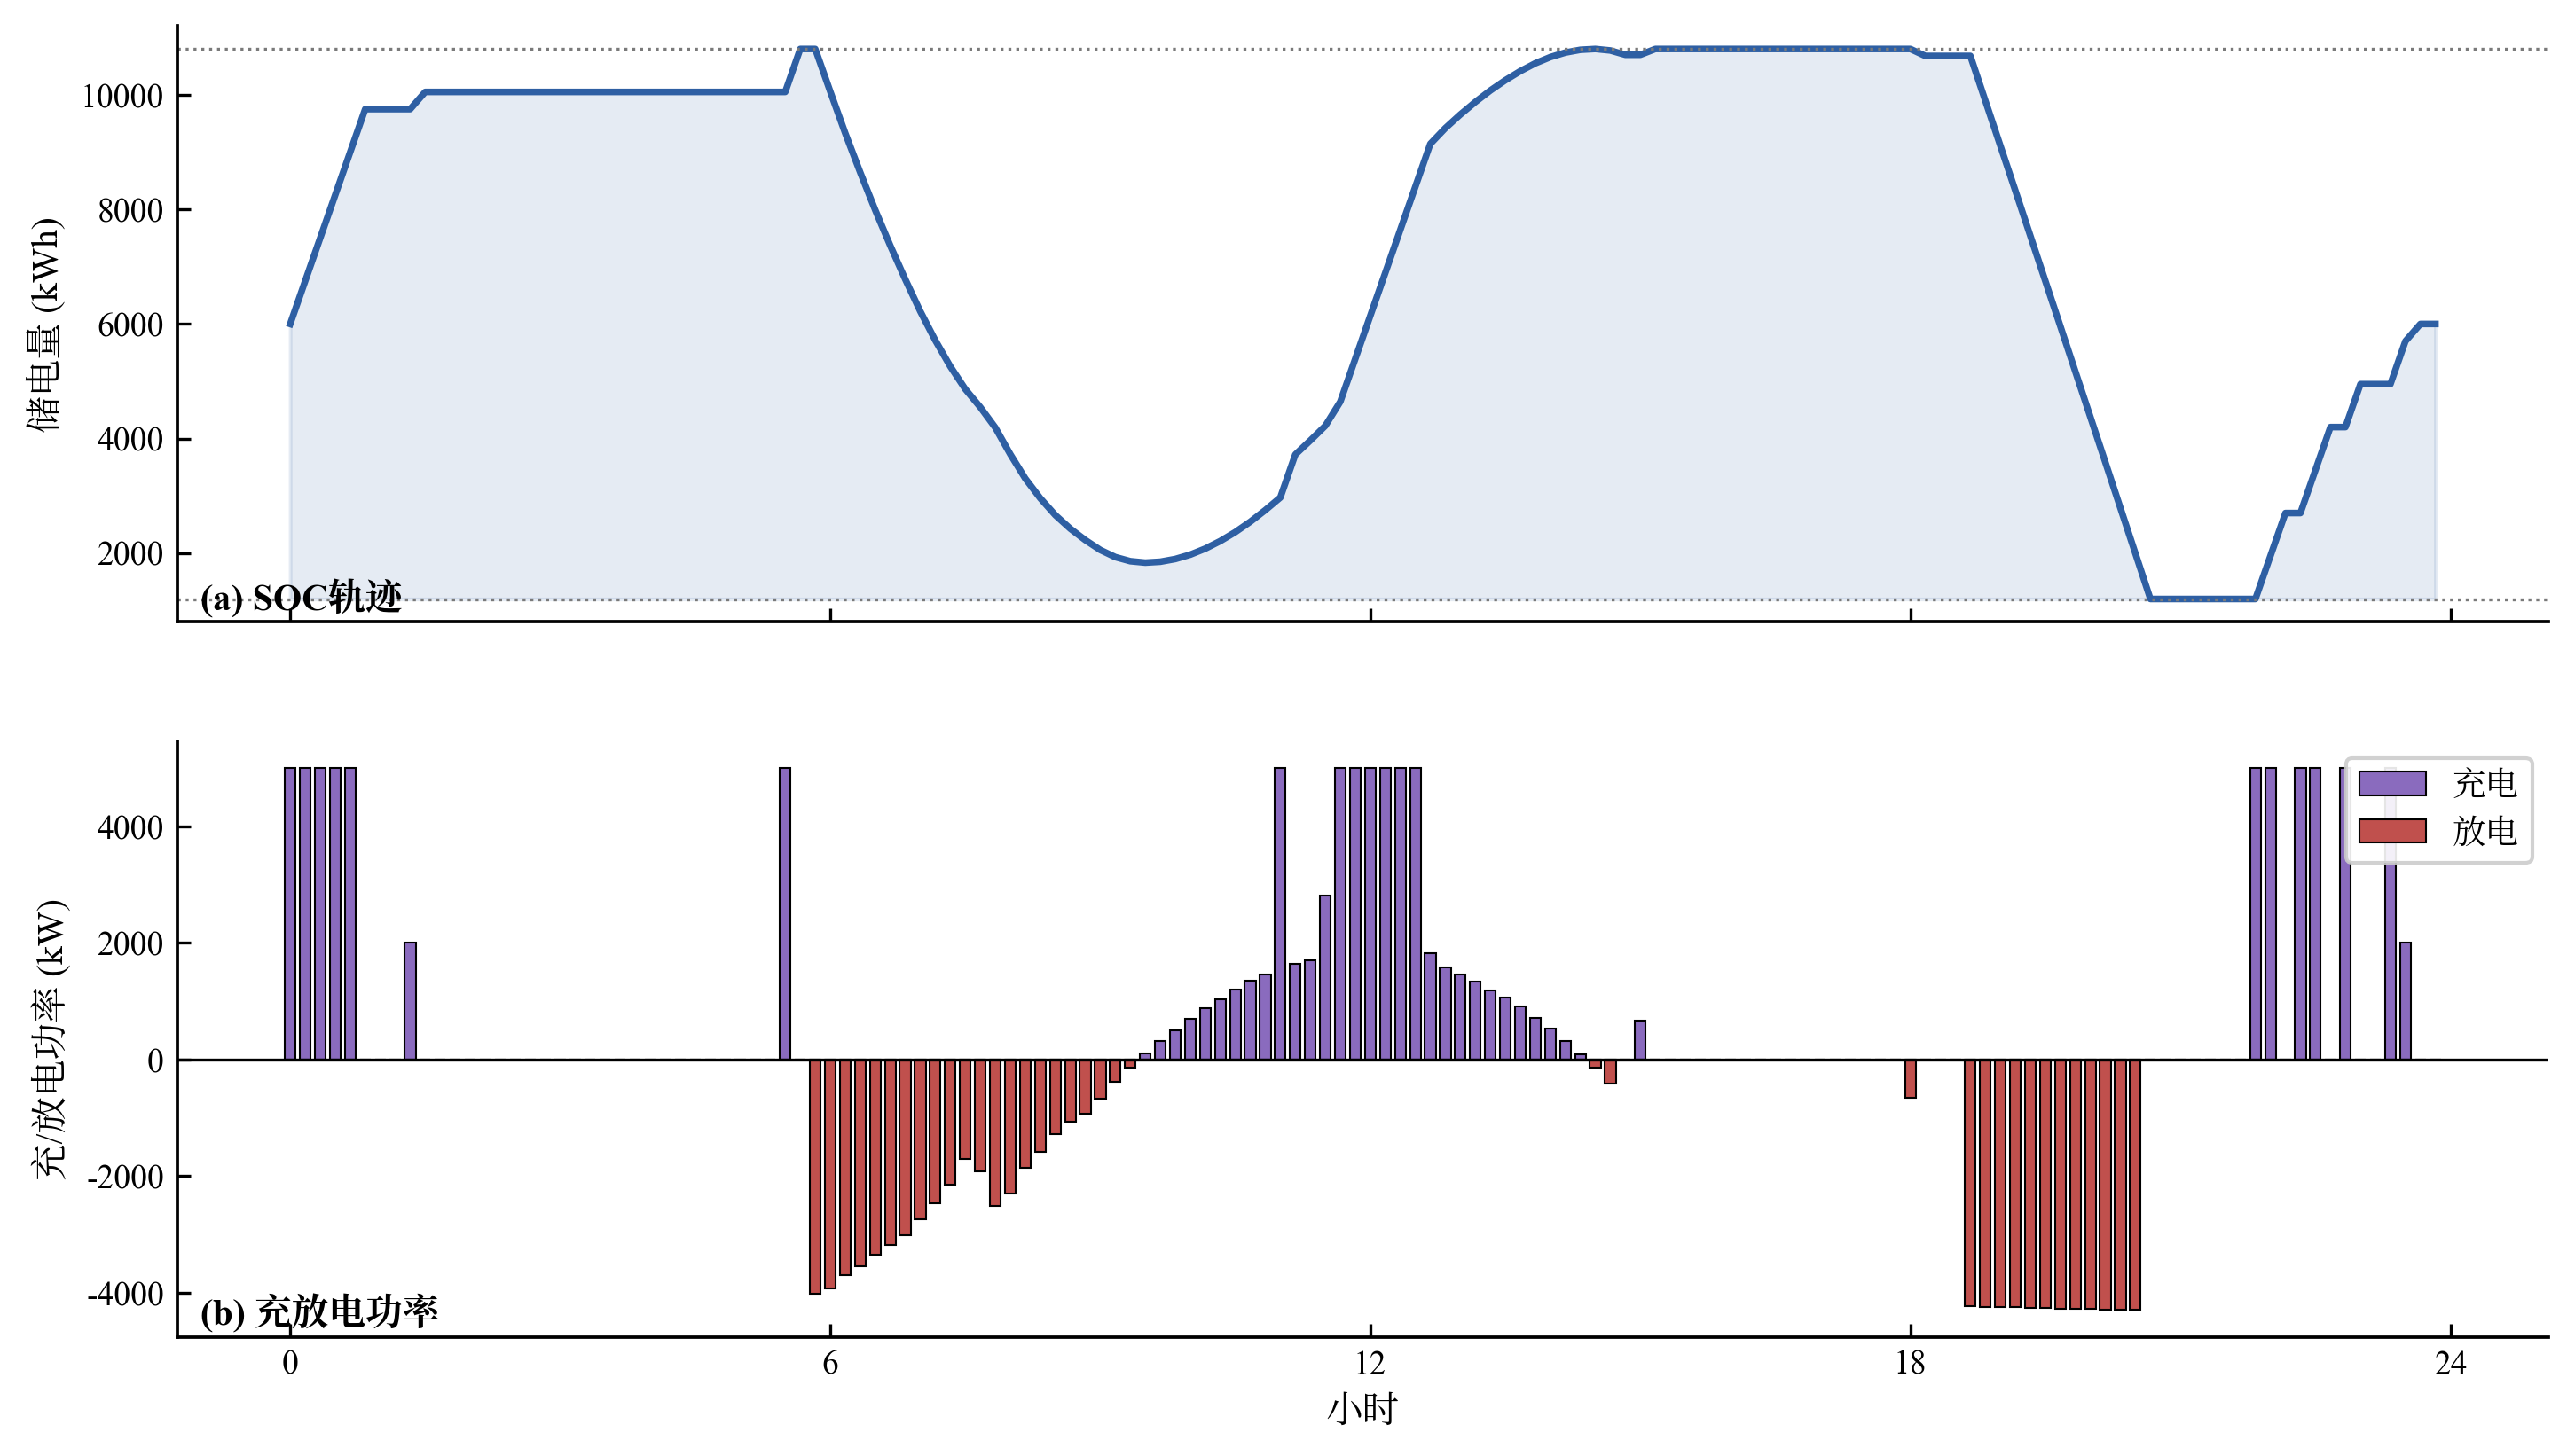
\includegraphics[width=0.62\textwidth]{求解/问题一/图片/图1-4_储能SOC与充放电功率.png}
    \caption{储能荷电状态轨迹与充放电功率}
    \label{fig:结果1-4}
\end{figure}

微网一天内的能量平衡关系如图\ref{fig:结果1-5}所示，购电、光伏与储能放电三类供给叠加后恰好覆盖小区负载与储能充电需求，任意时刻能量收支闭合，验证了功率平衡约束的严格满足。

\begin{figure}[H]
    \centering
    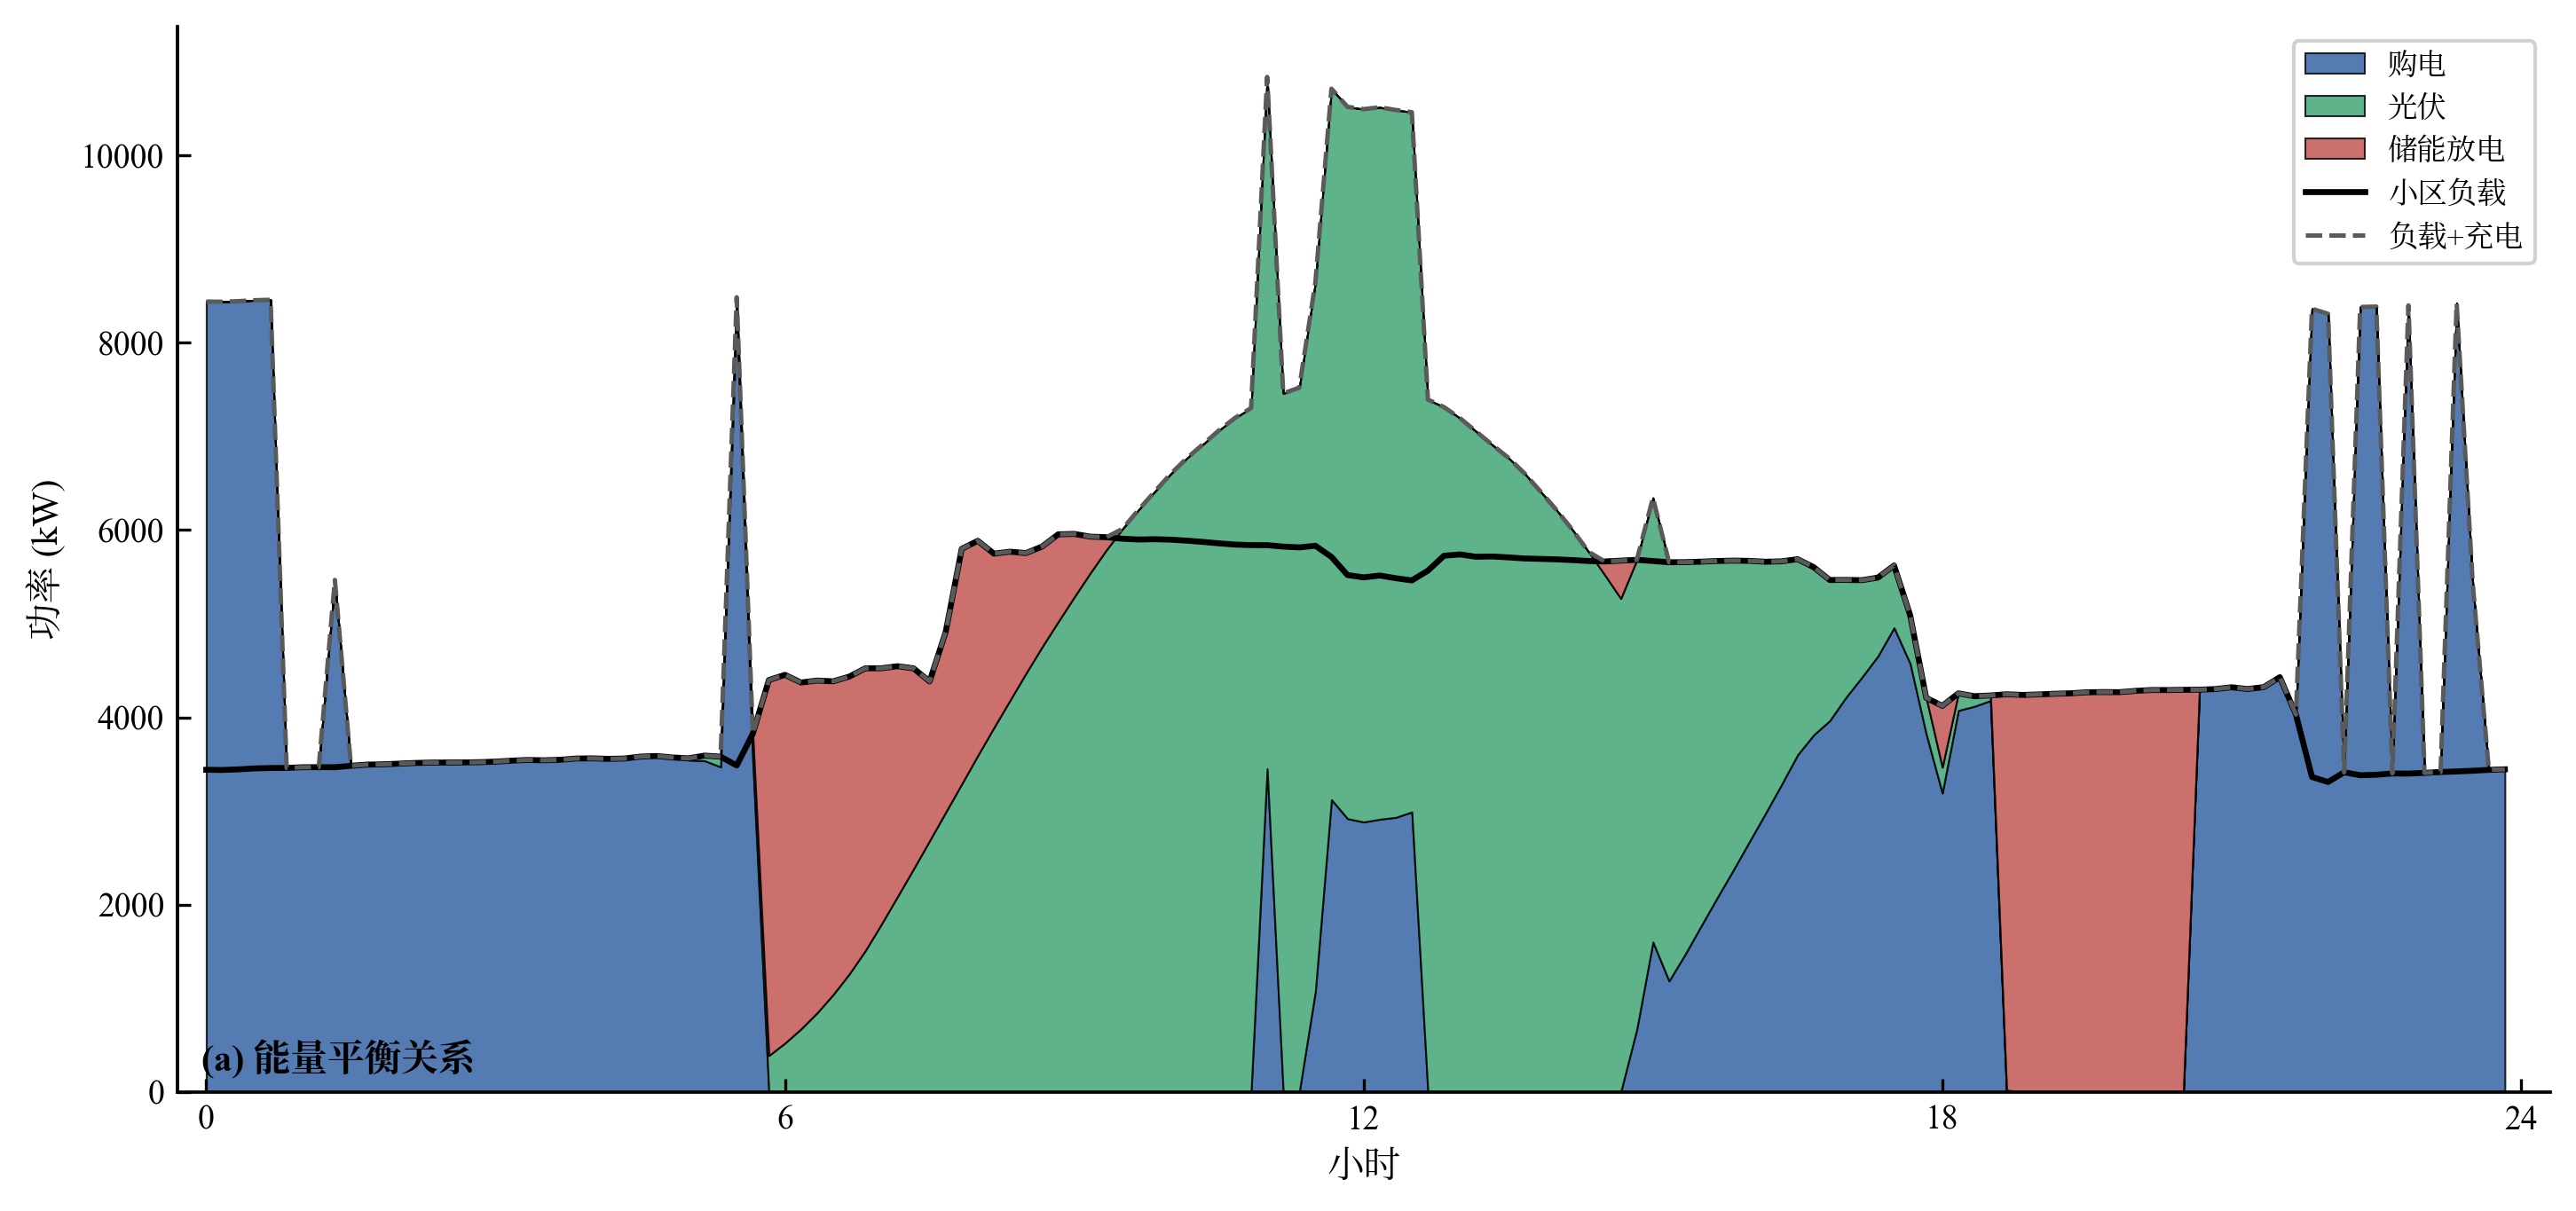
\includegraphics[width=0.70\textwidth]{求解/问题一/图片/图1-5_能量平衡.png}
    \caption{微网全天能量平衡关系}
    \label{fig:结果1-5}
\end{figure}

储能 0:00 储电量 $E_0$ 由附录1给定为 6000 kWh，属于问题给定的固定条件而非可优化变量。为进一步检验模型对该初值的稳健性，将 $E_0$ 在 $[1200,10800]$ kWh 区间内逐档变动（并保持日循环 $E_{144}=E_0$）重新求解全天购电费，结果如图\ref{fig:结果1-6}所示。可见购电费随 $E_0$ 变化总体平稳，在附录1给定的 6000 kWh 处购电费为 35126.95 元，与最低购电费相比差异很小，说明模型结果对储能初值的选取不敏感，也表明按给定初值求解是合理可靠的。

\begin{figure}[H]
    \centering
    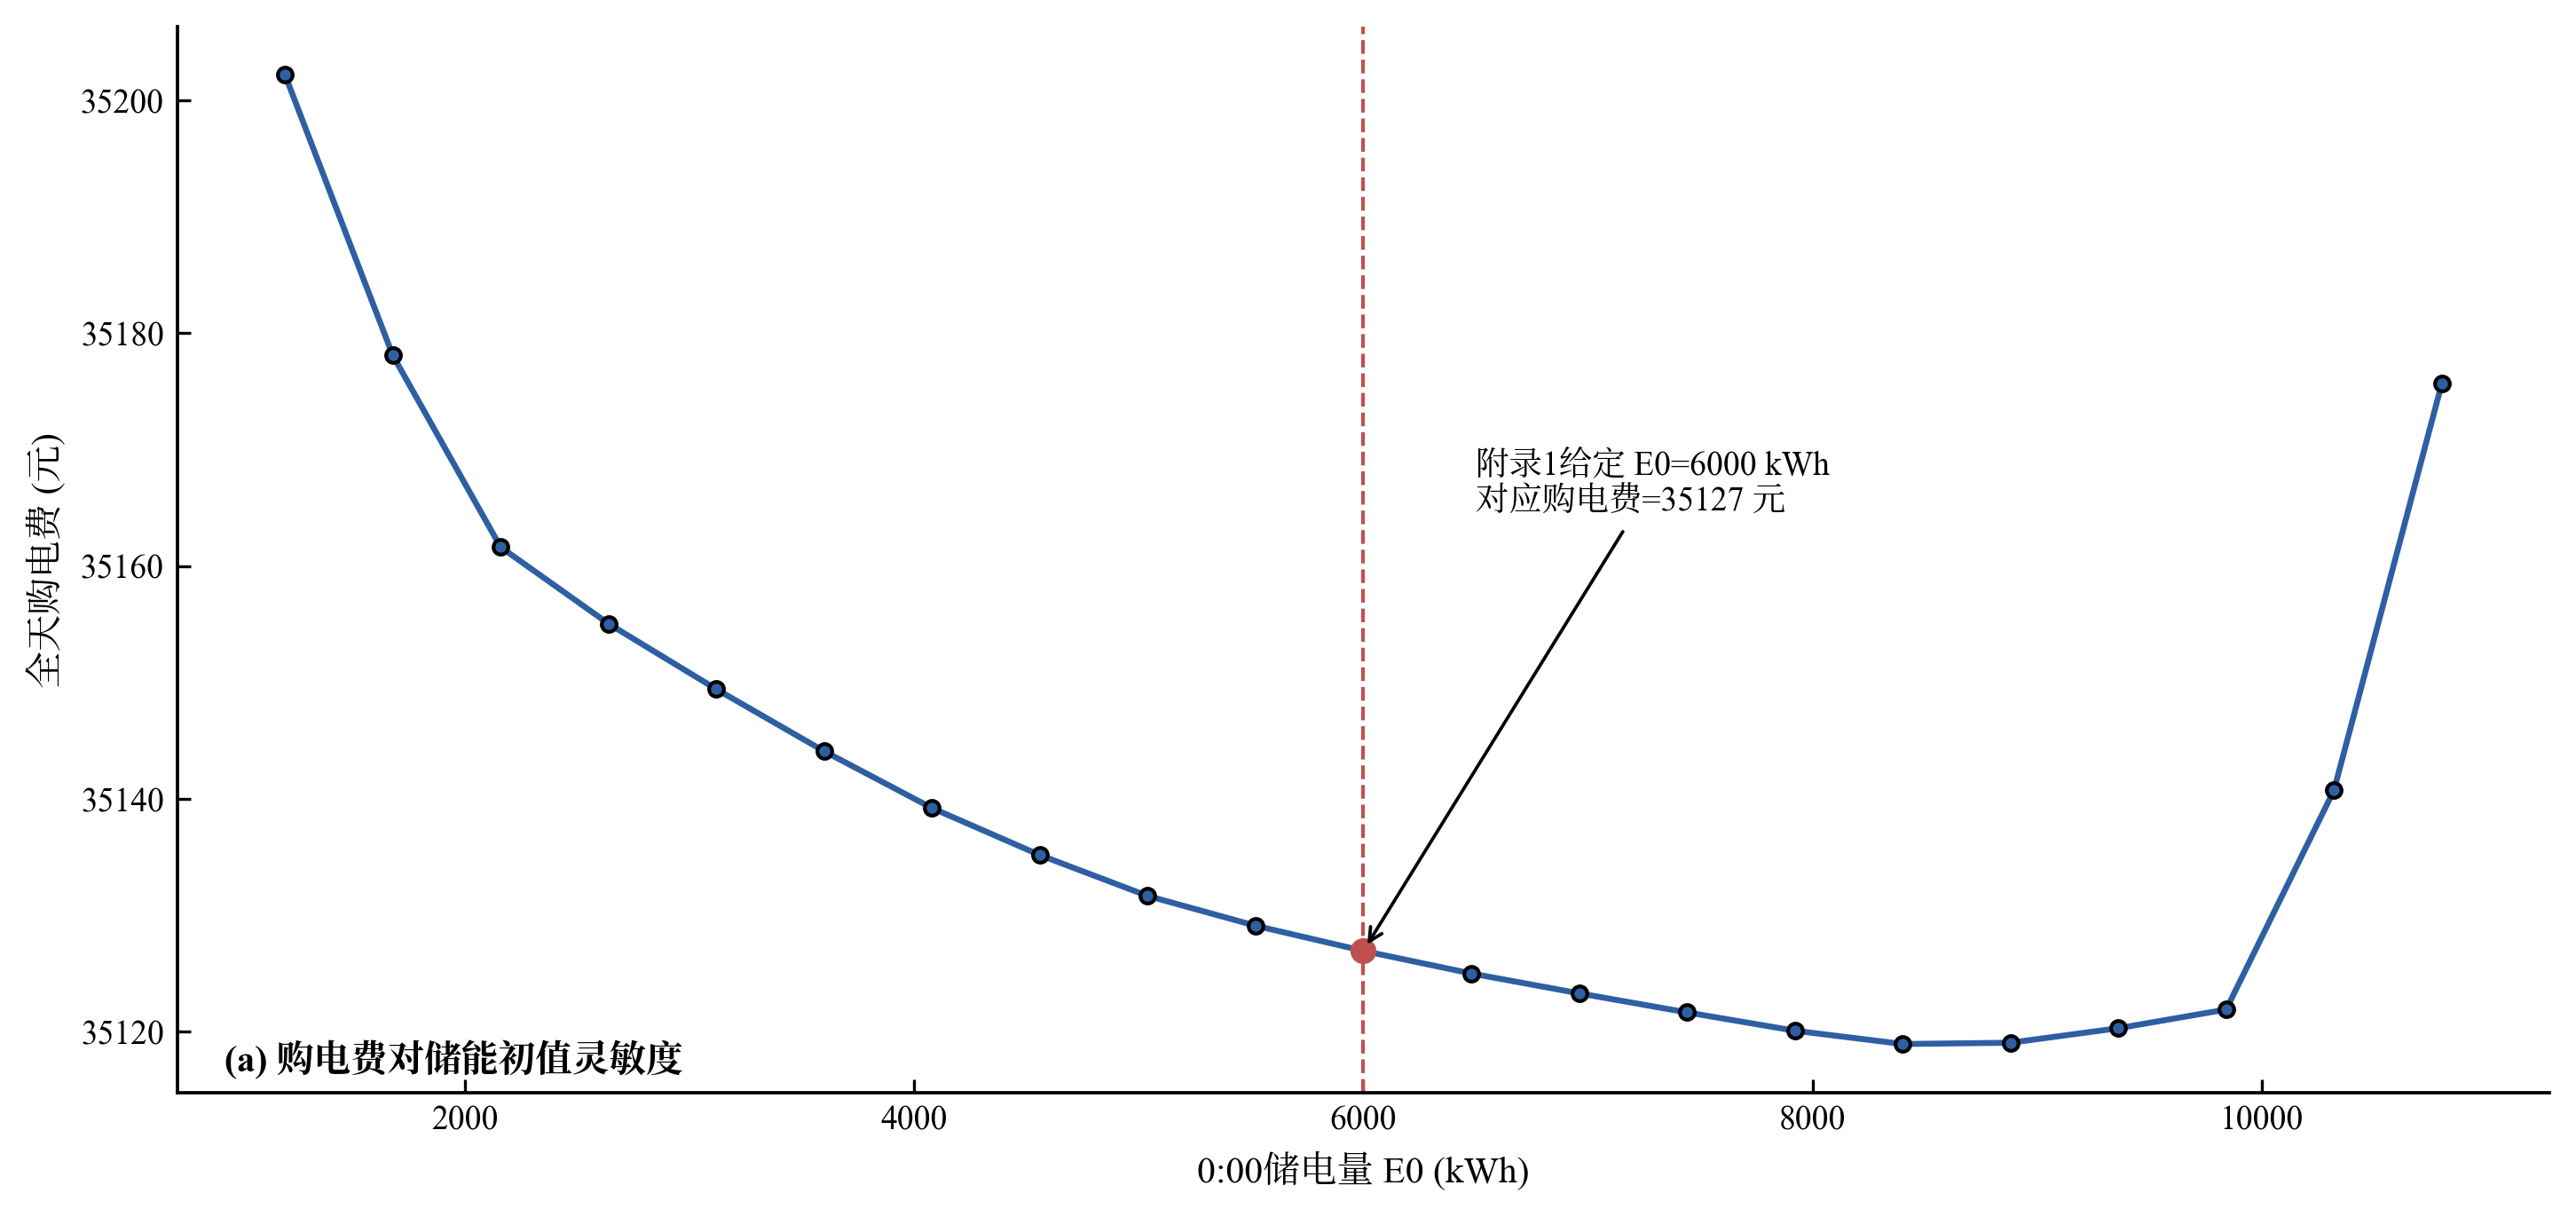
\includegraphics[width=0.70\textwidth]{求解/问题一/图片/图1-6_购电费灵敏度.png}
    \caption{全天购电费对储能初值的灵敏度}
    \label{fig:结果1-6}
\end{figure}

\begin{longtable}{>{\centering\arraybackslash}p{0.15\textwidth}>{\centering\arraybackslash}p{0.13\textwidth}>{\centering\arraybackslash}p{0.15\textwidth}>{\centering\arraybackslash}p{0.13\textwidth}>{\centering\arraybackslash}p{0.15\textwidth}>{\centering\arraybackslash}p{0.13\textwidth}}
  \caption{微网在指定时间段的购电量（kWh）及全天的购电量和购电费（元）}
  \label{tab:结果1-1} \\
  \toprule
  时间段 & 购电量 & 时间段 & 购电量 & 时间段 & 购电量 \\
  \midrule
  \endfirsthead
  \caption{微网在指定时间段的购电量（kWh）及全天的购电量和购电费（元，续）} \\
  \toprule
  时间段 & 购电量 & 时间段 & 购电量 & 时间段 & 购电量 \\
  \midrule
  \endhead
  \bottomrule
  \endfoot
  10:00--10:10 & 0.00 & 12:00--12:10 & 480.41 & 14:00--14:10 & 0.00 \\
  16:00--16:10 & 445.43 & 18:00--18:10 & 531.89 & 20:00--20:10 & 0.00 \\
  全天购电量 & 59482.70 & 全天购电费 & 35126.95 &  &  \\
\end{longtable}

\begin{longtable}{>{\centering\arraybackslash}p{0.15\textwidth}>{\centering\arraybackslash}p{0.13\textwidth}>{\centering\arraybackslash}p{0.13\textwidth}>{\centering\arraybackslash}p{0.15\textwidth}>{\centering\arraybackslash}p{0.13\textwidth}>{\centering\arraybackslash}p{0.13\textwidth}}
  \caption{储能设备在指定时间段的充放电量（kWh）及0:00和24:00的储电量（kWh）}
  \label{tab:结果1-2} \\
  \toprule
  时间段 & 充电量 & 放电量 & 时间段 & 充电量 & 放电量 \\
  \midrule
  \endfirsthead
  \caption{储能设备在指定时间段的充放电量（kWh）及0:00和24:00的储电量（kWh，续）} \\
  \toprule
  时间段 & 充电量 & 放电量 & 时间段 & 充电量 & 放电量 \\
  \midrule
  \endhead
  \bottomrule
  \endfoot
  0:00--4:00 & 4500.00 & 0.00 & 4:00--8:00 & 833.33 & 6365.84 \\
  8:00--12:00 & 4787.96 & 1703.00 & 12:00--16:00 & 5286.04 & 91.10 \\
  16:00--20:00 & 0.00 & 5780.13 & 20:00--24:00 & 5333.33 & 2859.87 \\
  0:00储电量 & 6000.00 &  & 24:00储电量 & 6000.00 &  \\
\end{longtable}

由表\ref{tab:结果1-1}可知，微网全天计划购电量为 59482.70 kWh，全天购电费为 35126.95 元；在 10:00--10:10、14:00--14:10 与 20:00--20:10 等光伏充足或储能放电充足的时段购电量为零，而在 12:00--12:10、16:00--16:10、18:00--18:10 等负荷高企时段需要少量购电。由表\ref{tab:结果1-2}可知，储能设备在 0:00 与 24:00 的储电量均为 6000.00 kWh，与附录1给定的 0:00 储电量一致，同时满足日循环约束；储能主要在 0:00--4:00、8:00--12:00 与 20:00--24:00 等低电价时段充电，在 4:00--8:00、16:00--20:00 等高电价时段放电，体现了低充高放的套利规律。

综观全天策略，购电出现在电价与光伏出力配合最有利的时段，储能则承担把低价电量搬运到高价时段的角色。这一分工使全天购电费用降至 35126.95 元，同时首末储电量同为 6000.00 kWh，满足日循环要求。
